% This is a LaTeX thesis template for Adam Mickiewicz University.
% to be used with Rmarkdown
% This template was produced by Jakub Nowosad
% Version: 16 February 2020

% Inspired by:
% This is a LaTeX thesis template for Monash University.
% to be used with Rmarkdown
% This template was produced by Rob Hyndman
% Version: 6 September 2016

\documentclass{amuthesis}
%\usepackage[polish]{babel}
%\usepackage{polski}
%\renewcommand{\figurename}{Figure} % Redefine default figure caption %
%\renewcommand{\tablename}{Table} % Redefine default table caption %
%%%%%%%%%%%%%%%%%%%%%%%%%%%%%%%%%%%%%%%%%%%%%%%%%%%%%%%%%%%%%%%
% Add any LaTeX packages and other preamble here if required
%%%%%%%%%%%%%%%%%%%%%%%%%%%%%%%%%%%%%%%%%%%%%%%%%%%%%%%%%%%%%%%
\usepackage{booktabs,tabularx} % Allows kableExtra to work %
\usepackage{indentfirst} % Adds indent in the first paragraph %
\usepackage{bookmark} % Adds indent in the first paragraph %

\author{Tomasz Matuszek}
\title{Measuring impact of Landsat 8 thermal band on supervised land
cover classification results}
\def\titleeng{Ocena wpływu zastosowania kanału termalnego Landsat na
wyniki nadzorowanej klasyfikacji pokrycia terenu}
\def\degreetitle{Engineer's Thesis}
\def\major{Geoinformation}
\def\albumid{455828}
\def\thesisyear{2023}
% Add subject and keywords below
\hypersetup{
     %pdfsubject={The Subject},
     %pdfkeywords={Some Keywords},
     pdfauthor={Tomasz Matuszek},
     pdftitle={Measuring impact of Landsat 8 thermal band on supervised
land cover classification results},
     pdfproducer={quarto with LaTeX}
}

\bibliography{thesis,packages}

\begin{document}

\pagenumbering{arabic}

\titlepage

\bookmarksetup{startatroot}

\hypertarget{abstract}{%
\chapter*{Abstract}\label{abstract}}
\addcontentsline{toc}{chapter}{Abstract}

\textbf{Abstrakt}

Streszczenie powinno przedstawiać skrótowo główny problem pracy i jego
rozwiązanie. Możliwa struktura streszczenia to: (1) 1-3 zdania wstępu do
problemu (czym się zajmujemy, dlaczego jest to ważne, jakie są
problemy/luki do wypełnienia), (2) 1 zdanie opisujące cel pracy, (3) 1-3
zdania przedstawiające użyte materiały (dane) i metody (techniki,
narzędzia), (4) 1-3 zdania obrazujące główne wyniki pracy, (5) 1-2
zdania podsumowujące; możliwe jest też określenie dalszych
kroków/planów.

Słowa kluczowe: (4-6 słów/zwrotów opisujących treść pracy, które nie
wystąpiły w tytule)

\textbf{Abstract}

The abstract must be consistent with the above text.

Keywords: (as stated before)

\newpage

\setstretch{1.2}\sf\tighttoc\doublespacing

\bookmarksetup{startatroot}

\hypertarget{sec-intro}{%
\chapter{Introduction}\label{sec-intro}}

\begin{itemize}
\item
  applications and relevance of land cover maps
\item
  machine learning and supervised classification of satellite images as
  a tool for creating land cover maps
\item
  pointing out that thermal band if often omitted in land cover
  classification models, exact impact of thermal factor isn't fully
  clear
\item
  goal of the thesis is to create land cover map of Poznań metropolitan
  area and measure the impact of thermal band on the model results
\end{itemize}

\begin{center}\rule{0.5\linewidth}{0.5pt}\end{center}

Wprowadzenie powinno mieć charakter opisu od ogółu do szczegółu (np.
trzy-pięć paragrafów). Pierwszy paragraf powinien być najbardziej
ogólny, a kolejne powinny przybliżać czytelnika do problemu.
Przedostatni paragraf powinien określić jaki jest problem (są problemy),
który praca ma rozwiązać i dlaczego jest to (są one) ważne.

Wprowadzenie powinno być zakończone stwierdzeniem celu pracy. Dodatkowo
tutaj może znaleźć się również krótki opis co zostało zrealizowane w
pracy.

Pisząc ten rozdział proszę pomyśleć o osobach, które zupełnie nie znają
opisywanej tematyki. Należy tutaj krok po kroku wyjaśnić podstawowe
koncepcje, istotność problemu, wyniki poprzednich podobnych badań, itd.
Ten rozdział obejmuje tylko kwestie, które już zostały wykonane przez
inne osoby - nowe wyniki mają swoje miejsce w rozdziale
\textbf{?@sec-wyniki}.

Każda kwestia opisana w tym rozdziale powinna być cytowana. Dodatnie
cytowania odbywa się poprzez uzupełnienie pliku \texttt{thesis.bib}
zapisem w formacie BibTeX, a następnie dodanie nazwy referencji
poprzedzonej znakiem \texttt{@}. Przykładowo, zacytowanie książki
Geocomputation with R odbywa się poprzez
\autocite{lovelace_geocomputation_2019}.

W przypadku, gdy cytowanie zostało poprawnie wpisane oraz istnieje w
pliku \texttt{thesis.bib} to bibliografia powinna się automatycznie
wygenerować na końcu pracy.

W przypadku, gdy praca dyplomowa opisuje konkretny obszar to można po
tym rozdziale stworzyć kolejny rozdział opisujący ``obszar badań''.

Ten i kolejne rozdziału moją mieć także podrozdziały. Tworzenie
podrozdziałów polega na stworzeniu nowej linii rozpoczynającej się od
znaków \texttt{\#\#} a następnie tytułu podrozdziału. Dodatkowo w
postaci \texttt{\{\#sec-\}} można dodać skrót nazwy
rozdziału/podrozdziału umożliwiający odnoszenie się do niego używając
operatora \texttt{{[}-@sec{]}}.

\bookmarksetup{startatroot}

\hypertarget{sec-data}{%
\chapter{Source data}\label{sec-data}}

Landsat ARD dataset, provided by GLAD laboratory at the Univeristy of
Maryland, was used in this study. Central-Western Poland was chosen as a
training area for which satellite imagery and land cover data were
downloaded (Figure \ref{fig-rycina1}). Training points were obtained
from LUCAS dataset created by Eurostat \autocite{dandrimont2020}. This
data was pre-processed and then used to train the model and validate its
performance.

\begin{figure}[t]

{\centering 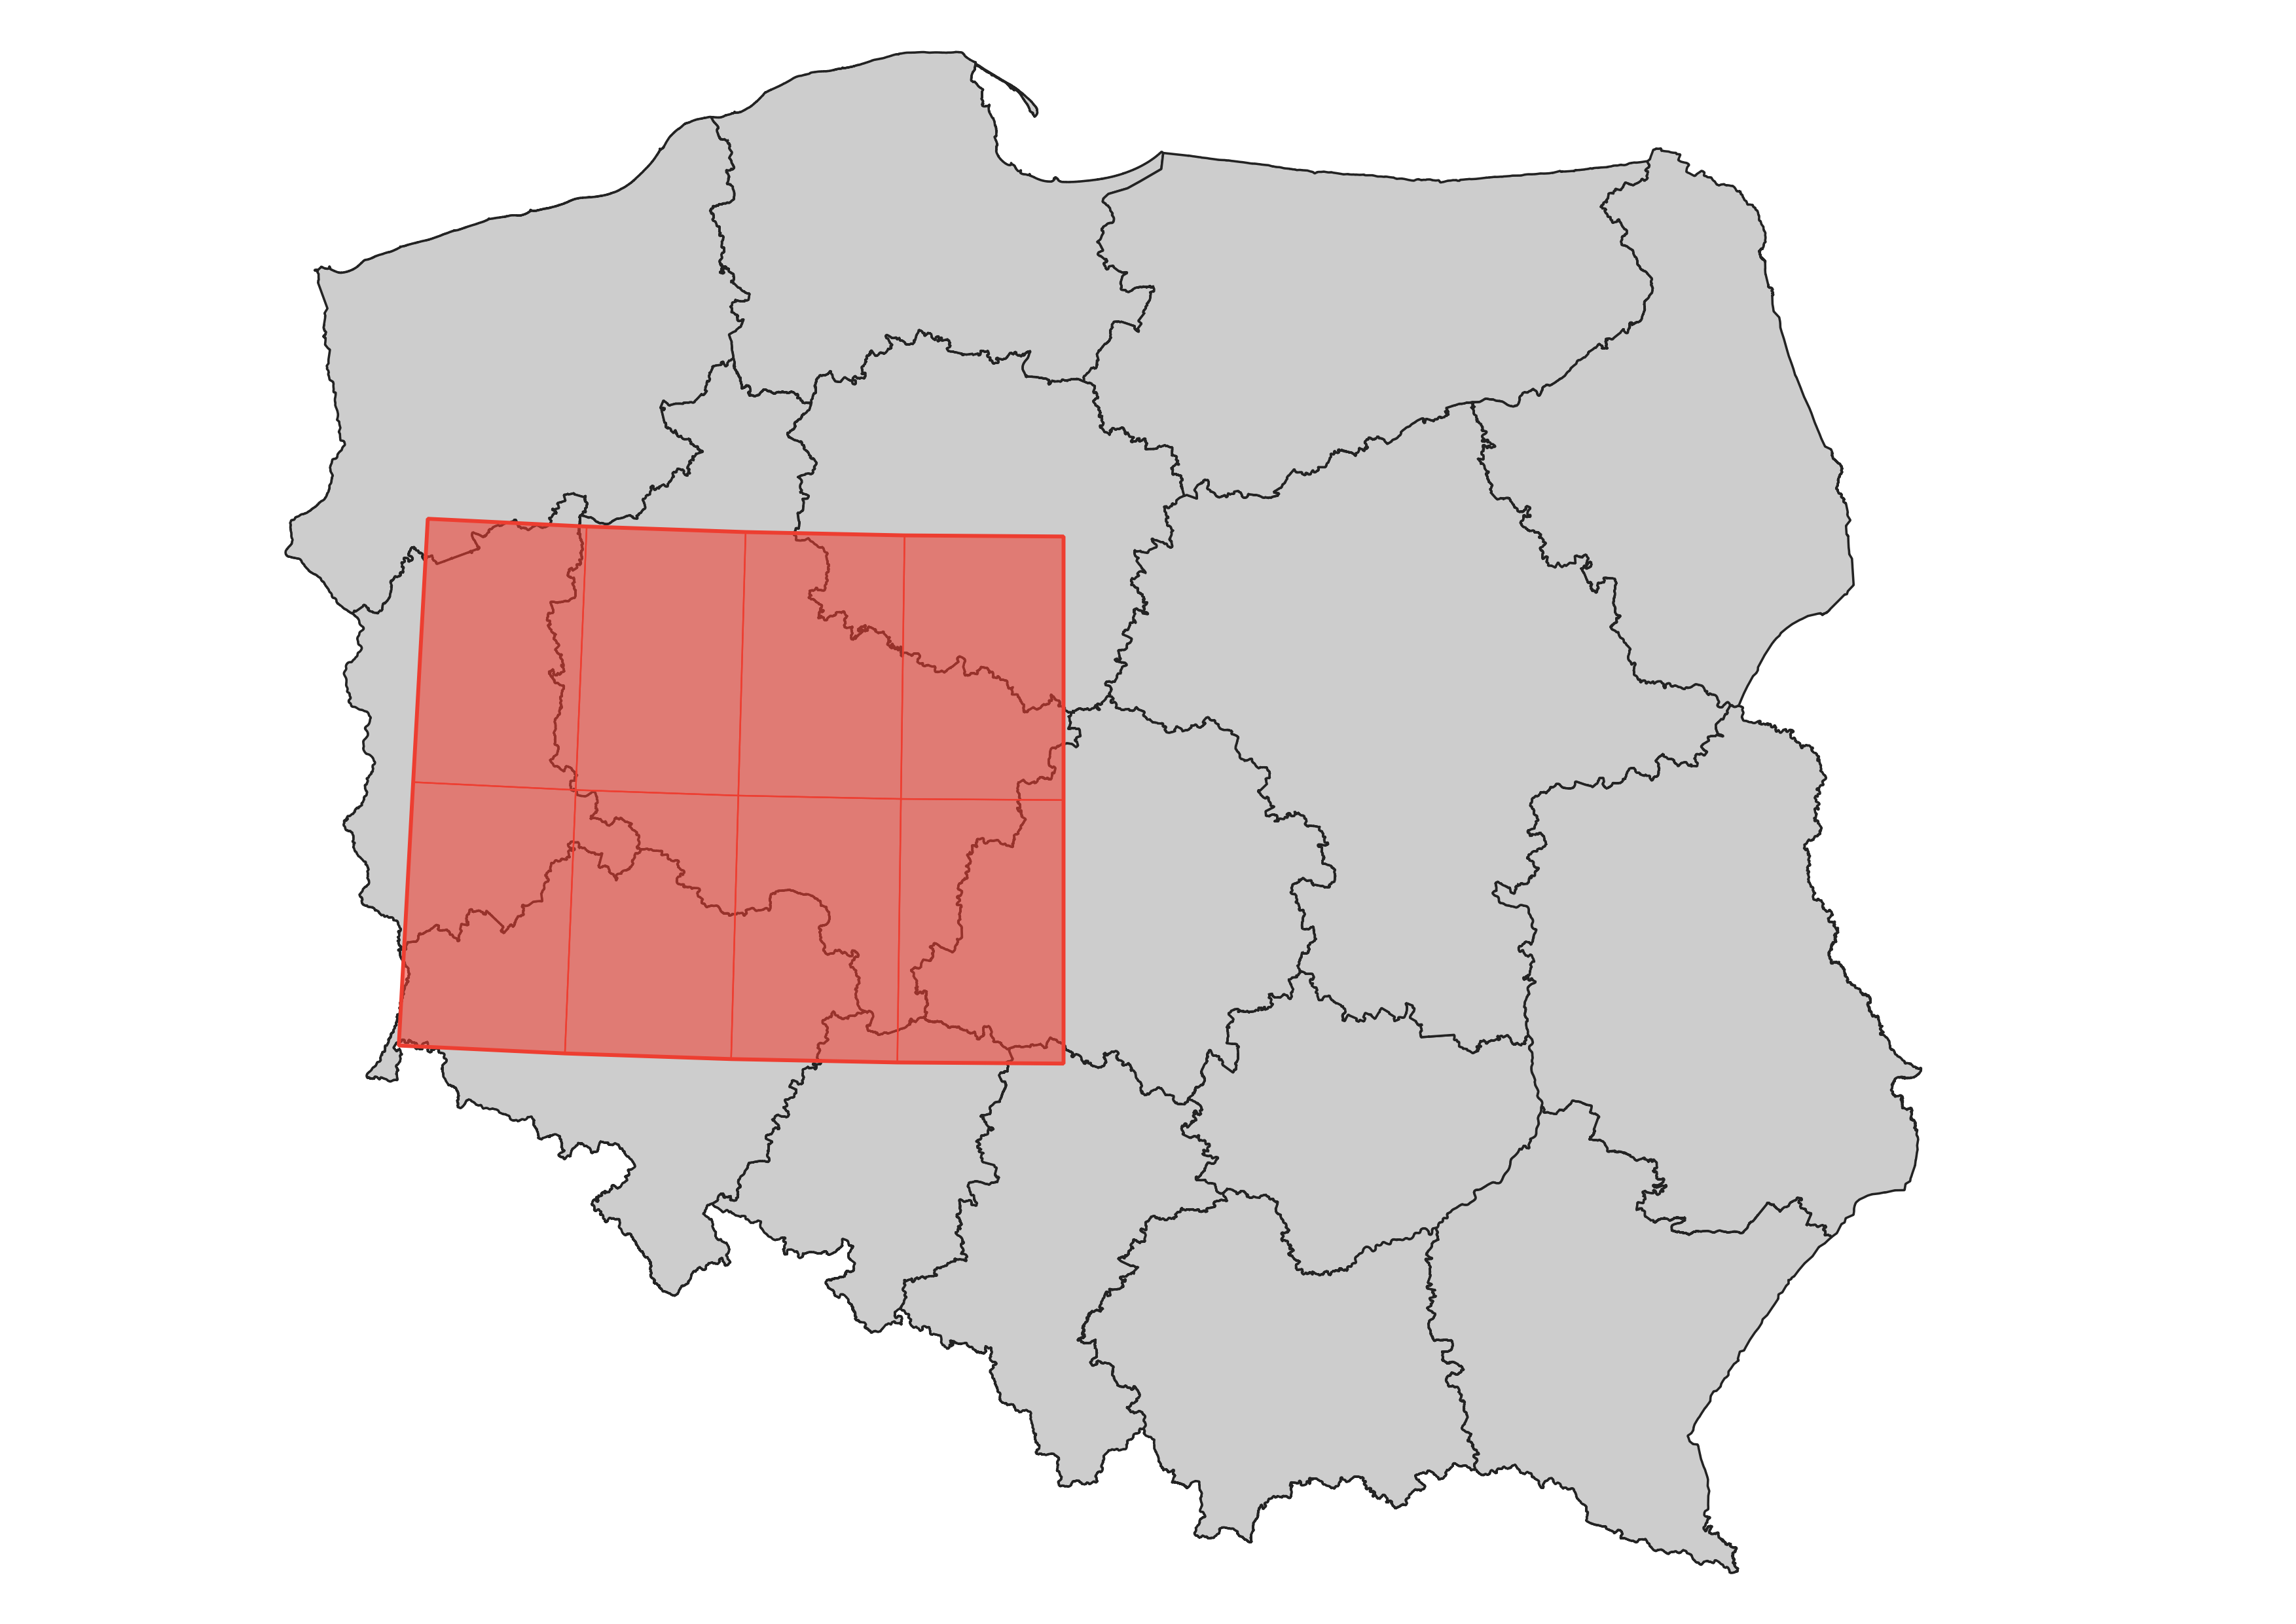
\includegraphics[width=1\textwidth,height=4.16667in]{./figures/study_area.png}

}

\caption{\label{fig-rycina1}Training area}

\end{figure}

\hypertarget{sec-sat}{%
\section{Satellite imagery}\label{sec-sat}}

Satellite imagery from GLAD Landsat ARD is available in 16-day interval
composites and is divided into 1° x 1° tiles. Processing of original
Landsat images performed by GLAD team included converting spectral bands
to top-of-atmosphere (TOA) reflectance, converting thermal band to
brightness temperature (BT) in Kelvins, scaling the values of all bands
as well as adding quality flag for every pixel \autocite{potapov2020}.

Satellite images for eight 1° x 1° tiles, covering the study area
(Figure \ref{fig-rycina1}), were downloaded using GLAD Tools v1.1 and
PERL programming language. These images are from 10th interval of the
year 2018, so downloaded mosaics consist of images created between
24.05.2018 and 8.06.2018. All downloaded images were merged and
reprojected from WGS84 coordinate reference system (EPSG:4326) to UTM
zone 33N (EPSG:32633). Every band was also resampled from 0.00025°
resolution (corresponding to 27.83 m on equator) to 30 meters
resolution.

In addition, four spectral indices were derived: Normalized Difference
Vegetation Index (NDVI), Modified Normalized Difference Water Index
(MNDWI), Normalized Difference Moisture Index (NDMI) and Modified Bare
soil Index (MBI). Formulas used to calculate these indices can be found
in Table \ref{tbl-tabela1}.

\hypertarget{tbl-tabela1}{}
\begin{table}
\caption{\label{tbl-tabela1}Formulas of spectral indices dervied from Landsat data }\tabularnewline

\centering
\begin{tabular}{>{\raggedright\arraybackslash}p{4cm}ll}
\toprule
\textbf{band/index} & \textbf{short name} & \textbf{formula}\\
\midrule
Blue & B2 & -\\
Green & B3 & -\\
Red & B4 & -\\
Near Infrared & B5 (NIR) & -\\
Short-wave Infrared 1 & B6 (SWIR1) & -\\
\addlinespace
Short-wave Infrared 2 & B7 (SWIR2) & -\\
Thermal & B10 (TIRS1) & -\\
Normalized Difference Vegetation Index & NDVI & (B5 -B4) / (B4 + B5)\\
Modified Normalized Difference Water Index & MNDWI & (B3 - B6) / (B3 + B6)\\
Normalized Difference Moisture Index & NDMI & (B5 - B6) / (B5 + B6)\\
\addlinespace
Modified Bare Surface Index & MBI & (B6 - B7 - B5) / (B6 + B7 + B5) + 0.5\\
\bottomrule
\end{tabular}
\end{table}

\hypertarget{sec-landcover}{%
\section{Land cover data}\label{sec-landcover}}

Data collected during LUCAS survey performed by Eurostat was chosen as
land cover training set. At the moment of writing, it is the most
accurate and comprehensive dataset containing information about land use
and land cover \autocite{pflugmacher2019} due to the fact, that every
point was either manually photo-interpreted or assessed during
\emph{in-situ} visit.

LUCAS survey consists of two phases. First phase is based on grid of
points with 2km spacing covering whole territory of the European Union
(which equals to more than 1 million points). Each point of the grid is
visually interpreted using ortho-photos or satellite images, and
classified into one of seven major land-cover classes. These classes
are: arable land, permanent crops, grassland, wooded areas/shrub land,
bare land, artificial land and water. In the second phase, a subsample
of grid points is selected and then visited by Eurostat surveyors. They
classify each point according to full LUCAS land cover and land use
classification. The survey takes place in the spring and summer in order
to observe chosen places in high vegetation season
\autocite{dandrimont2020}.

Surveyor not only assign land cover and land use classes to points, but
they also add auxillary information such as plant species present at the
site, percentage of land coverage for a chosen class, height of the
trees and their maturity, as well as information about water management
and irrigation. If there are more than one land cover/land use types at
the point, observer can also assign a secondary class for every LUCAS
point.

Majority of the training points used for the classification model were
points from the second phase of LUCAS survey, also called LUCAS Primary
Data. We downloaded a total of 4,153 points for the study area.
Pre-processing step included omitting records with missing data,
excluding artificial linear land cover classes (e.g.~roads or railways)
and excluding points that were surveyed more than 500 meters from their
theoretical location. In the next step, detailed land cover classes were
aggregated into eight main groups of land cover types. Two of them -
grassland and shrubland were additionally aggregated into one land cover
class. Then, we filtered some of the classes according to the percentage
of land coverage or percentage of impervious surface coverage (Table
\ref{tbl-tabela2}).

\hypertarget{tbl-tabela2}{}
\begin{table}
\caption{\label{tbl-tabela2}Filters applied to reclassified land cover groups. IMP - impervious
surface, HERB - herbaceous plants cover, TC - tree cover }\tabularnewline

\centering
\begin{tabular}{lll>{\raggedright\arraybackslash}p{4cm}>{\raggedright\arraybackslash}p{3cm}}
\toprule
\textbf{ID} & \textbf{LC class} & \textbf{LUCAS Grid} & \textbf{LUCAS Primary Data} & \textbf{Applied filters}\\
\midrule
1 & arable land & - & B00 (Cropland) & <30\% IMP\\
2 & grasslands & - & E00 (Grassland), D00 (Shrubland) & >50\% HERB; <30\% IMP\\
3 & forests & - & C00 (Woodland) & >50\% TC; <20\% IMP\\
4 & bare land & 6 (Bare surface) & F00 (Bare land) & -\\
5 & artificial land & 7 (Artificial areas) & A00 (Artificial land) & >70\% IMP\\
\addlinespace
6 & water bodies & 8 (Inland water) & G00 (Water areas) & -\\
7 & wetlands & - & H00 (Wetlands) & -\\
\bottomrule
\end{tabular}
\end{table}

For the least frequent classes in the LUCAS Primary Data dataset - bare
land, artificial land and water bodies - we also added points classified
during the first phase of LUCAS survey (Figure \ref{fig-rycina2}). This
step was necessary to ensure that every land cover class is represented
by enough number of points. It was not possible only for wetlands class,
because of lack of such category in the first phase classification. At
the end of the pre-processing, we were left with 3,778 training points
\autocite{oliverbuck2015}.

\begin{figure}[t]

{\centering 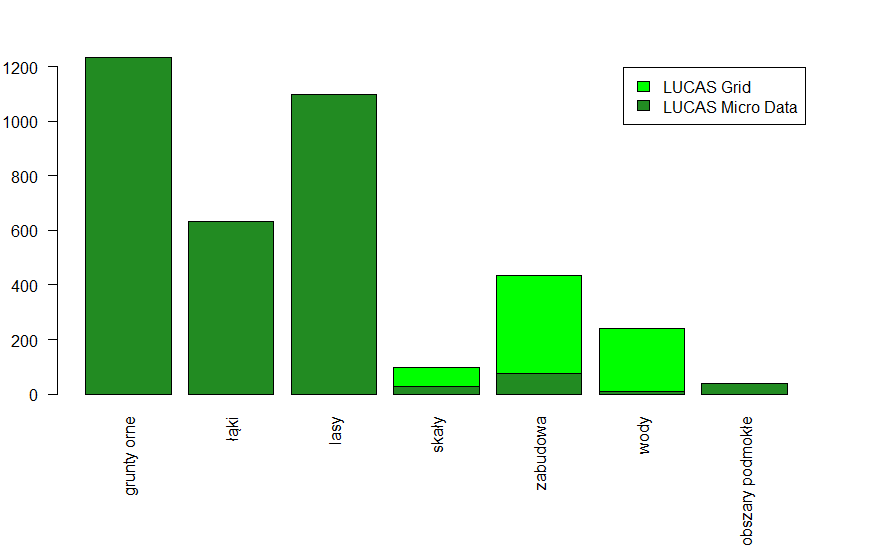
\includegraphics[width=1\textwidth,height=3.64583in]{./figures/lucas_data.png}

}

\caption{\label{fig-rycina2}Distribution of land cover classes after
pre-processing}

\end{figure}

After extracting values from Landsat ARD raster, LUCAS points were also
filtered using quality flag provided. Only points with clear-sky quality
flag were taken into account during the process of model training. We
also excluded water bodies points in which NDWI was lower than 0. These
two conditions excluded over 400 points in total.

Training set obtained after pre-processing can be seen in Figure
\ref{fig-rycina3}. Spatial distribution of data points was fairly even
and due to the structure of LUCAS data set, every point was located at
least 2 kilometers from another one.

\begin{figure}[t]

{\centering 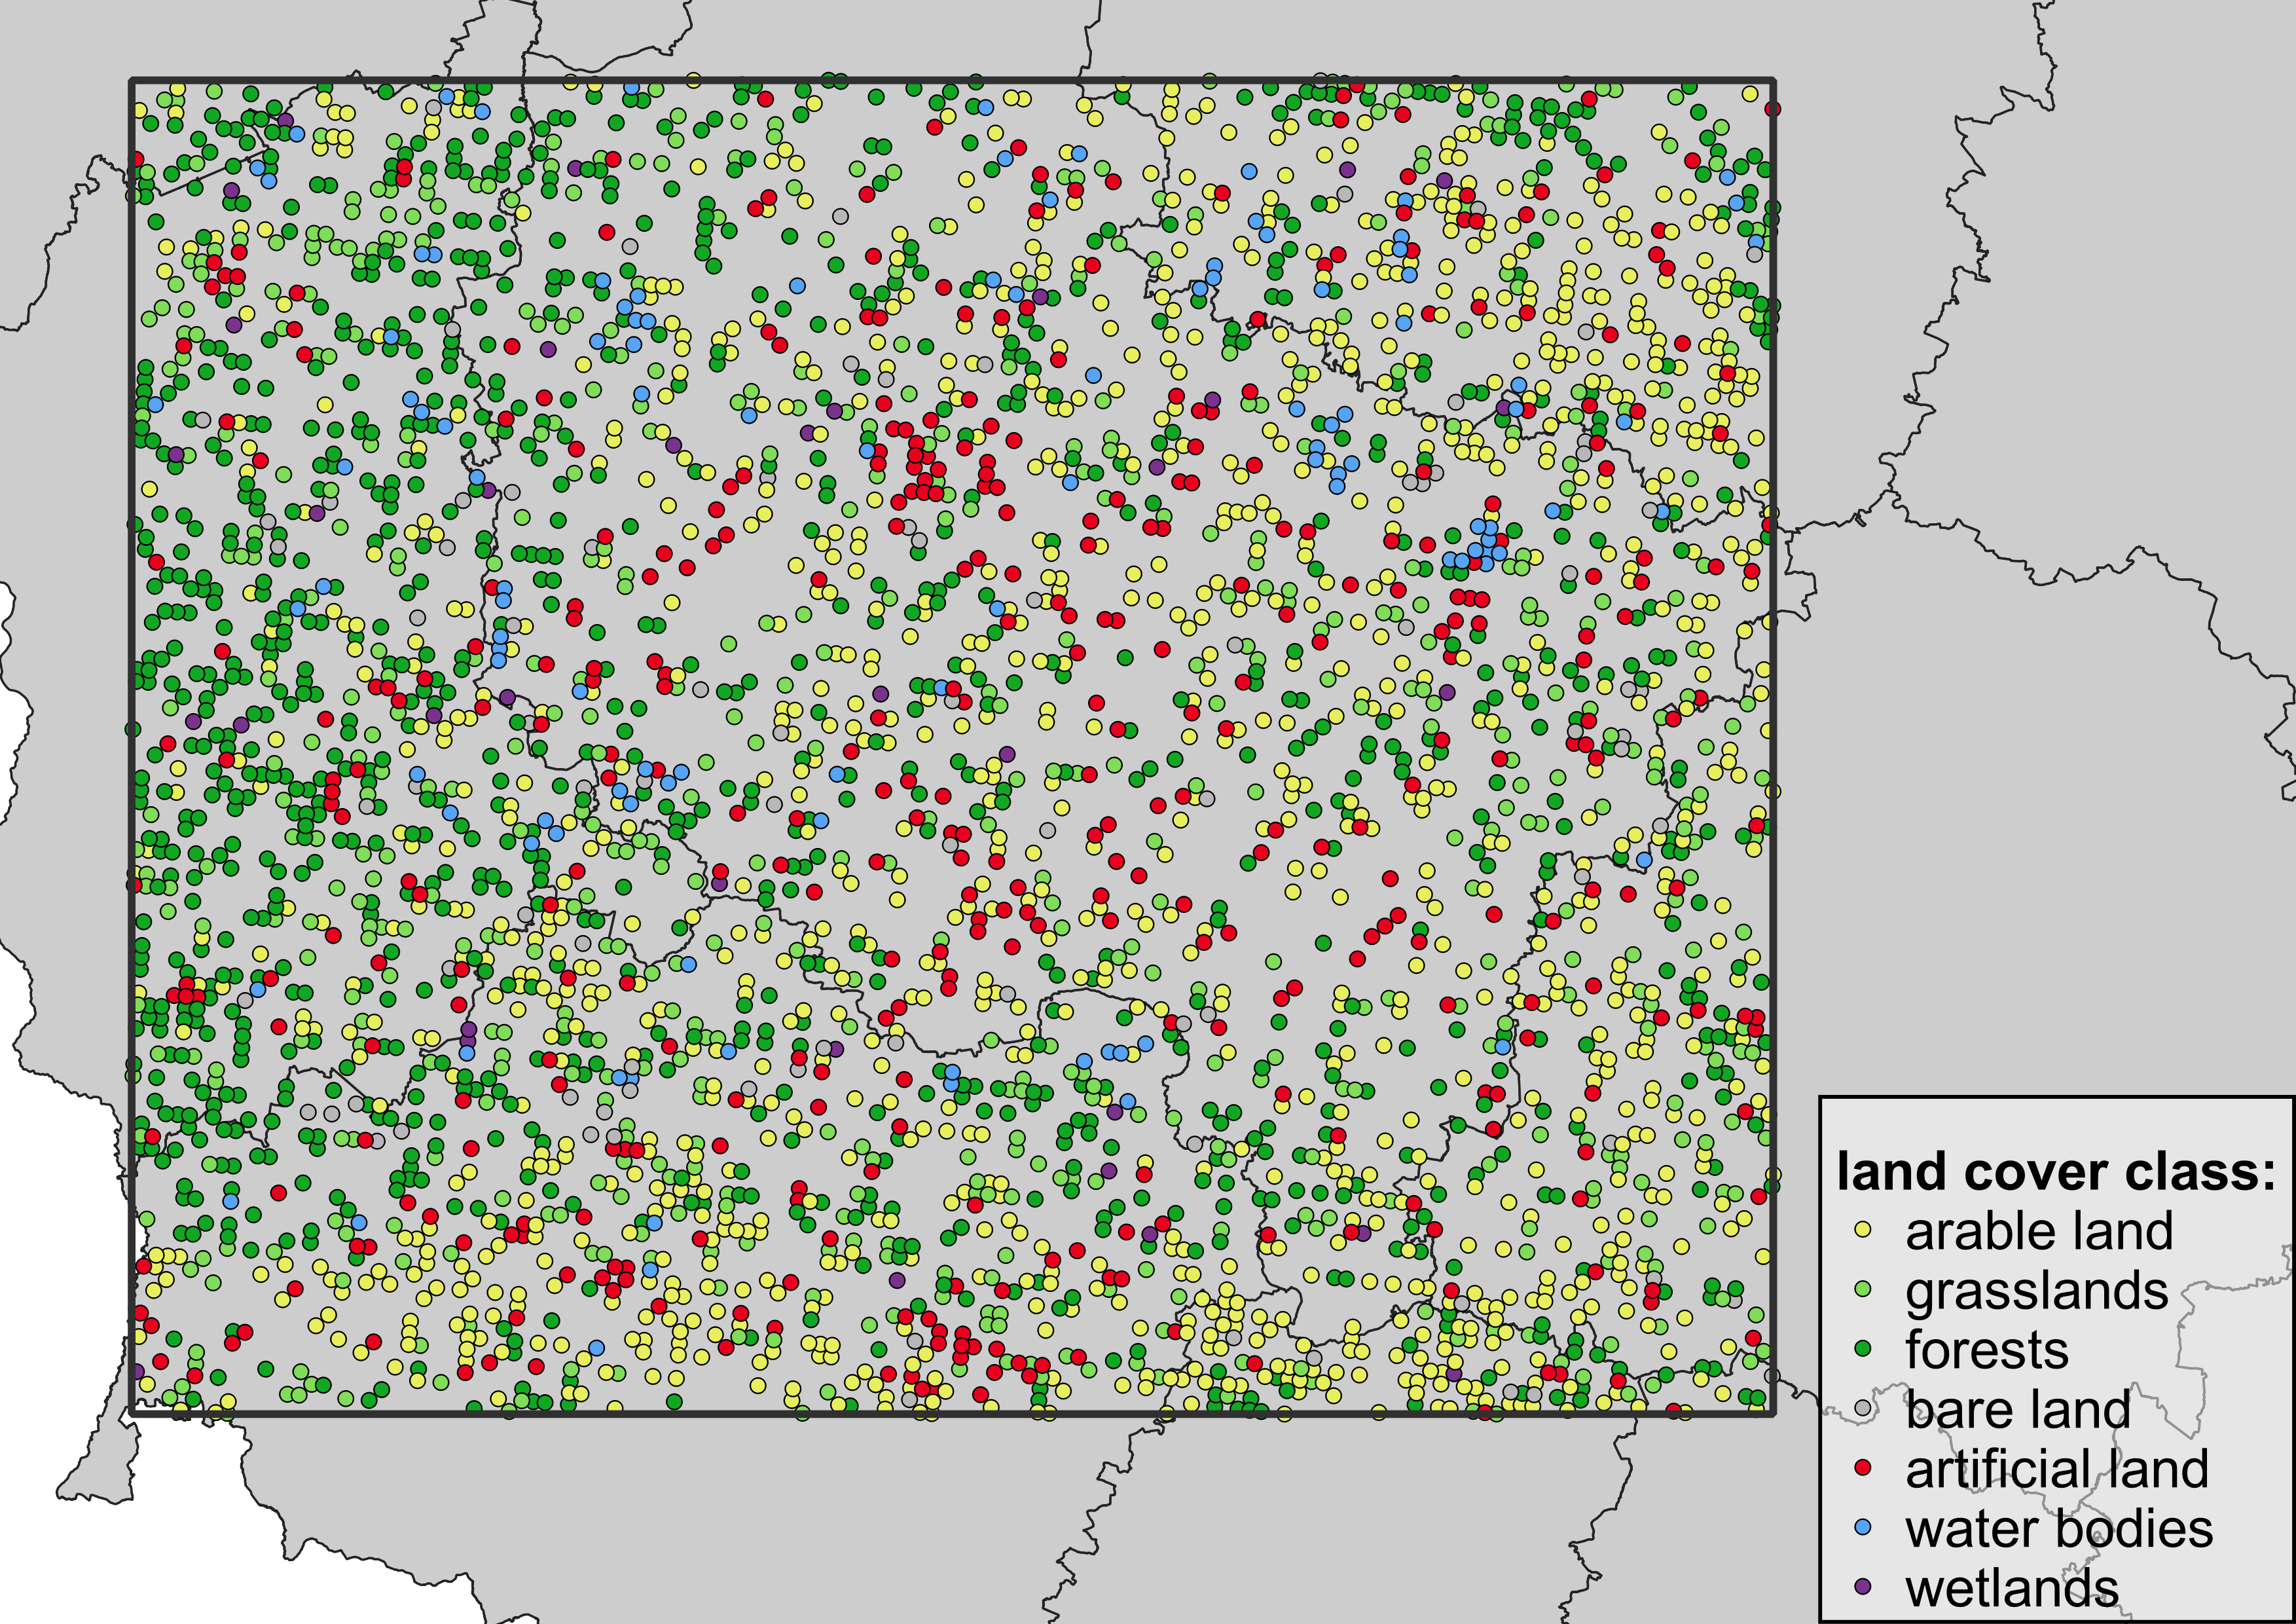
\includegraphics[width=1\textwidth,height=4.16667in]{./figures/lucas_distribution.png}

}

\caption{\label{fig-rycina3}Spatial distribution of LUCAS training
points after pre-processing}

\end{figure}

\bookmarksetup{startatroot}

\hypertarget{sec-methods}{%
\chapter{Methods}\label{sec-methods}}

\hypertarget{sec-ml}{%
\section{Machine learning}\label{sec-ml}}

\begin{itemize}
\item
  what is machine learning and what are its applications
\item
  classification vs regression algorithms
\item
  supervised and unsupervised classification
\end{itemize}

\hypertarget{sec-rf}{%
\subsection{Random forest algorithm}\label{sec-rf}}

\begin{itemize}
\item
  what is a decision tree
\item
  how random forest algorithm works
\end{itemize}

\hypertarget{sec-resampling}{%
\subsection{Model quality assessment}\label{sec-resampling}}

\begin{itemize}
\item
  idea of resampling
\item
  measures and indices of classification model quality
\end{itemize}

\hypertarget{sec-tuning}{%
\subsection{Parameter tuning}\label{sec-tuning}}

\begin{itemize}
\item
  what is tuning of model's parameters
\item
  idea of nested resampling
\end{itemize}

\hypertarget{sec-r}{%
\section{R language environment}\label{sec-r}}

Short description of R and RStudio environment. List of used libraries
and packages.

\begin{center}\rule{0.5\linewidth}{0.5pt}\end{center}

Rozdział \textbf{Metody} zawiera opis użytych metod (np. statystycznych
czy geostatystycznych) oraz technologii (np. pakiety R). Opis każdej z
metod czy technologi powinien być zwarty i zawierać tylko najważniejsze
informacje z punktu widzenia pracy dyplomowej.

Każda użyta metoda i technologia powinna być zacytowana. W przypadku
pakietów R, wystarczy wypełnić poniższy blok kodu (zwróć uwagę, że ten
blok kodu ma parametr \texttt{echo:\ false}; oznacza to, że będzie on
niewidoczny w wynikowym pliku PDF)\ldots{}

\ldots{} a następnie zacytować pakiet używając znaku \texttt{@}, po
którym podać nazwę pakietu rozpoczynającą się od prefiksu \texttt{R-}.
Przykładowe cytowanie języka R bez nawiasu to \textcite{R-base}, a
pakietu \textbf{kableExtra} w nawiasie to \autocite{R-kableExtra}.
Więcej przykładów cytowania można znaleźć na stronie
https://rmarkdown.rstudio.com/authoring\_bibliographies\_and\_citations.html\#citations.

W przypadkach, gdy cytowanie istnieje, ale nie jest pakietem R to należy
dodać je do pliku \texttt{thesis.bib} i użyć powyższej składni ze
znakiem \texttt{@}. W ostateczności, gdy dana technologia nie posiada
cytowania, należy podać jej adres internetowy.

\bookmarksetup{startatroot}

\hypertarget{sec-results-map}{%
\chapter{Result of the model - land cover map}\label{sec-results-map}}

\begin{itemize}
\item
  land cover map of Poznań metropolitan area
\item
  probability map of model results
\end{itemize}

\begin{center}\rule{0.5\linewidth}{0.5pt}\end{center}

Część \textbf{Wyniki} może składać się z jednego lub więcej rozdziałów.
Każdy z tych rozdziałów powinien mieć tytuł adekwatny do swojej treści.

Rozdziały wynikowe powinny korzystać z wiedzy opisanej w poprzednich
rozdziałach (Rozdziały \textbf{?@sec-lit}, \textbf{?@sec-dane},
\textbf{?@sec-metody}). W przypadku prac analitycznych, ich treść
powinna przedstawiać kolejne etapy eksploracji i analizy danych. W
przypadku prac technicznych, treść tych rozdziałów powinna opisywać
stworzone narzędzia, a następnie pokazywać ich zastosowanie/a.

W przypadku prac technicznych warto pokazywać fragmenty napisanego
rozwiązania lub jego wywołania używając bloków kodu.

\begin{Shaded}
\begin{Highlighting}[]
\NormalTok{moja\_funkcja }\OtherTok{=} \ControlFlowTok{function}\NormalTok{(x)\{}
  \FunctionTok{cat}\NormalTok{(x, }\StringTok{"rządzi!"}\NormalTok{)}
\NormalTok{\}}
\FunctionTok{moja\_funkcja}\NormalTok{(}\StringTok{"Autor tej pracy"}\NormalTok{)}
\end{Highlighting}
\end{Shaded}

\begin{verbatim}
Autor tej pracy rządzi!
\end{verbatim}

\bookmarksetup{startatroot}

\hypertarget{sec-results-eval}{%
\chapter{Assessing model quality}\label{sec-results-eval}}

Table with quality indices:

\begin{itemize}
\item
  overall accuracy (OA)
\item
  classification error (CE)
\item
  producer's and user's accuracy (PA, UA)
\item
  Kappa coefficient
\end{itemize}

\begin{center}\rule{0.5\linewidth}{0.5pt}\end{center}

Część \textbf{Wyniki} może składać się z jednego lub więcej rozdziałów.
Każdy z tych rozdziałów powinien mieć tytuł adekwatny do swojej treści.

Rozdziały wynikowe powinny korzystać z wiedzy opisanej w poprzednich
rozdziałach (Rozdziały \textbf{?@sec-lit}, \textbf{?@sec-dane},
\textbf{?@sec-metody}). W przypadku prac analitycznych, ich treść
powinna przedstawiać kolejne etapy eksploracji i analizy danych. W
przypadku prac technicznych, treść tych rozdziałów powinna opisywać
stworzone narzędzia, a następnie pokazywać ich zastosowanie/a.

W przypadku prac technicznych warto pokazywać fragmenty napisanego
rozwiązania lub jego wywołania używając bloków kodu.

\begin{Shaded}
\begin{Highlighting}[]
\NormalTok{moja\_funkcja }\OtherTok{=} \ControlFlowTok{function}\NormalTok{(x)\{}
  \FunctionTok{cat}\NormalTok{(x, }\StringTok{"rządzi!"}\NormalTok{)}
\NormalTok{\}}
\FunctionTok{moja\_funkcja}\NormalTok{(}\StringTok{"Autor tej pracy"}\NormalTok{)}
\end{Highlighting}
\end{Shaded}

\begin{verbatim}
Autor tej pracy rządzi!
\end{verbatim}

\bookmarksetup{startatroot}

\hypertarget{sec-results-therm}{%
\chapter{Evaluation of thermal band's impact on prediction
results}\label{sec-results-therm}}

\begin{itemize}
\item
  mean temperature for every predicted land cover class
\item
  variable importance plots, variable profiles
\item
  thermal band importance map (two methods: raster aggregation and
  interpolation of importance in LUCAS points)
\item
  mean importance of thermal band on each land cover class
\item
  difference raster map between prediction with and without thermal band
  included, transition matrix
\end{itemize}

\begin{center}\rule{0.5\linewidth}{0.5pt}\end{center}

Część \textbf{Wyniki} może składać się z jednego lub więcej rozdziałów.
Każdy z tych rozdziałów powinien mieć tytuł adekwatny do swojej treści.

Rozdziały wynikowe powinny korzystać z wiedzy opisanej w poprzednich
rozdziałach (Rozdziały \textbf{?@sec-lit}, \textbf{?@sec-dane},
\textbf{?@sec-metody}). W przypadku prac analitycznych, ich treść
powinna przedstawiać kolejne etapy eksploracji i analizy danych. W
przypadku prac technicznych, treść tych rozdziałów powinna opisywać
stworzone narzędzia, a następnie pokazywać ich zastosowanie/a.

W przypadku prac technicznych warto pokazywać fragmenty napisanego
rozwiązania lub jego wywołania używając bloków kodu.

\begin{Shaded}
\begin{Highlighting}[]
\NormalTok{moja\_funkcja }\OtherTok{=} \ControlFlowTok{function}\NormalTok{(x)\{}
  \FunctionTok{cat}\NormalTok{(x, }\StringTok{"rządzi!"}\NormalTok{)}
\NormalTok{\}}
\FunctionTok{moja\_funkcja}\NormalTok{(}\StringTok{"Autor tej pracy"}\NormalTok{)}
\end{Highlighting}
\end{Shaded}

\begin{verbatim}
Autor tej pracy rządzi!
\end{verbatim}

\bookmarksetup{startatroot}

\hypertarget{conclusion}{%
\chapter{Conclusion}\label{conclusion}}

\begin{itemize}
\item
  land cover map of Poznań metropolitan area was created, impact of
  thermal band on classification results was measured
\item
  despite thermal band having low overall impact on model results, there
  is a strong spatial auto-correlation for its importance
\item
  land surface temperature was especially significant for land cover
  classification of urban areas, it helped in identify built-up areas
\item
  it may mean that thermal band will become increasingly important in
  studies on urban sprawl and suburbanisation
\item
  better land cover maps will help in better management of metropolitan
  areas growth and quantifying impact of urbanisation on natural
  environment more precisely
\end{itemize}

\begin{center}\rule{0.5\linewidth}{0.5pt}\end{center}

Podsumowanie pracy jest w pewnym sensie znacznie rozbudowanym
abstraktem. Należy wyliczyć i opisać osiągnięcia uzyskane w pracy
dyplomowej. Tutaj jednak (w przeciwieństwie do np. rozdziału
\textbf{?@sec-wprowadzenie}) należy przechodzić od szczegółu do ogółu -
co zostało stworzone/określone, jak zostało to zrobione, jakie ma to
konsekwencje, itd.

Ten rozdział powinien też zawierać opis kwestii, których nie udało się
rozwiązać w pracy dyplomowej (i dlaczego się nie udało) oraz pomysły na
przyszłe ulepszenie uzyskanych wyników lub dalsze badania.

\printbibliography[heading=bibintoc, title=Bibliography]

\end{document}
